\subsection{Interfejs}
Trzecia iteracja dogadywania szczegółów z klientem zawiera dodatkowy \textit{header} oraz przedstawione rozsunięte \textit{menu hamburger}.

\begin{figure}[H]
\centering
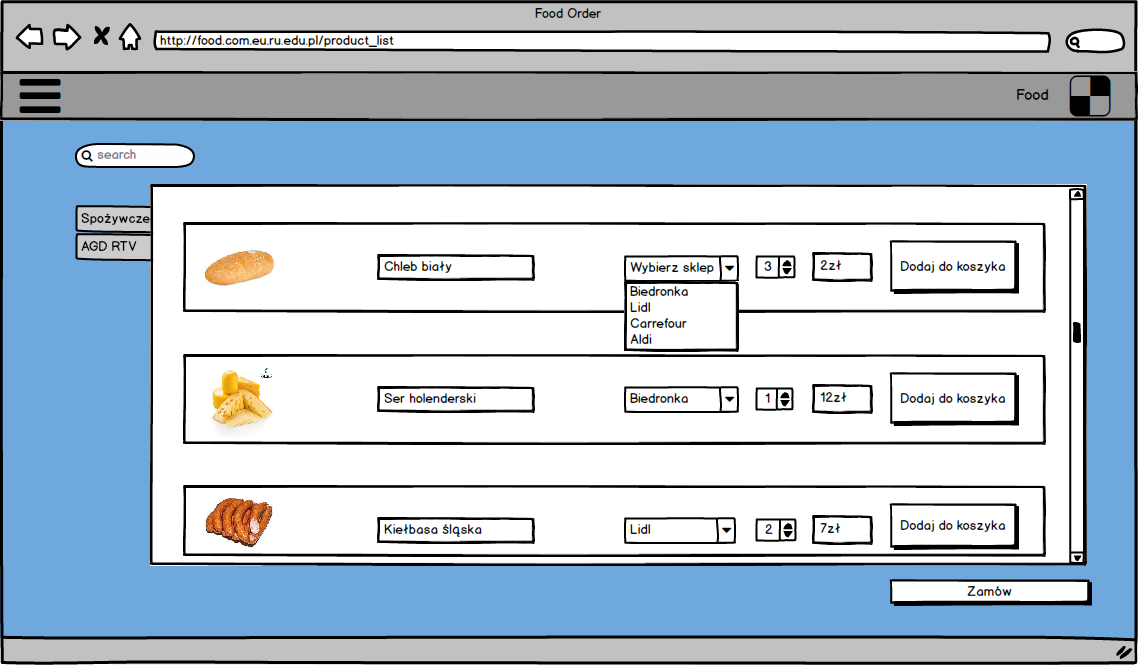
\includegraphics[width=15cm]{pictures/Lista_produktow_v3.png}
\caption{Trzecia iteracja wyboru listy produktów.}
\end{figure}

\begin{figure}[H]
\centering
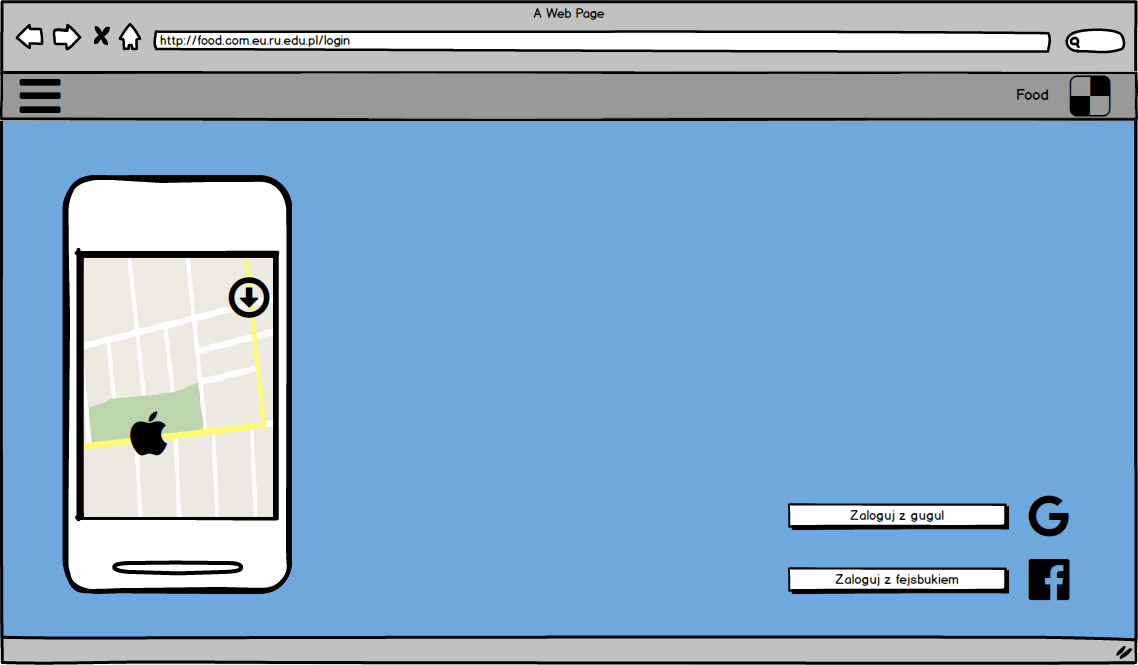
\includegraphics[width=15cm]{pictures/Logowanie_v1.png}
\caption{Ekran logowanie w trzeciej iteracji.}
\end{figure}

\begin{figure}[H]
\centering
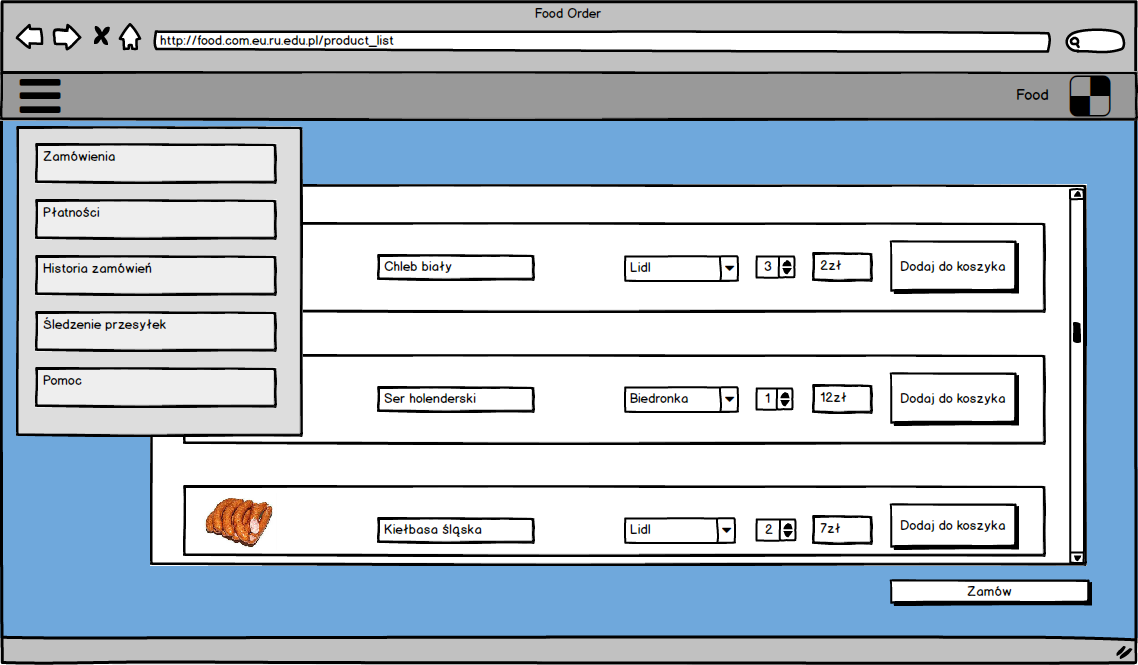
\includegraphics[width=15cm]{pictures/Navbar_v1.png}
\caption{Rozsunięte \textit{menu hamburger}.}
\end{figure}

\begin{figure}[H]
\centering
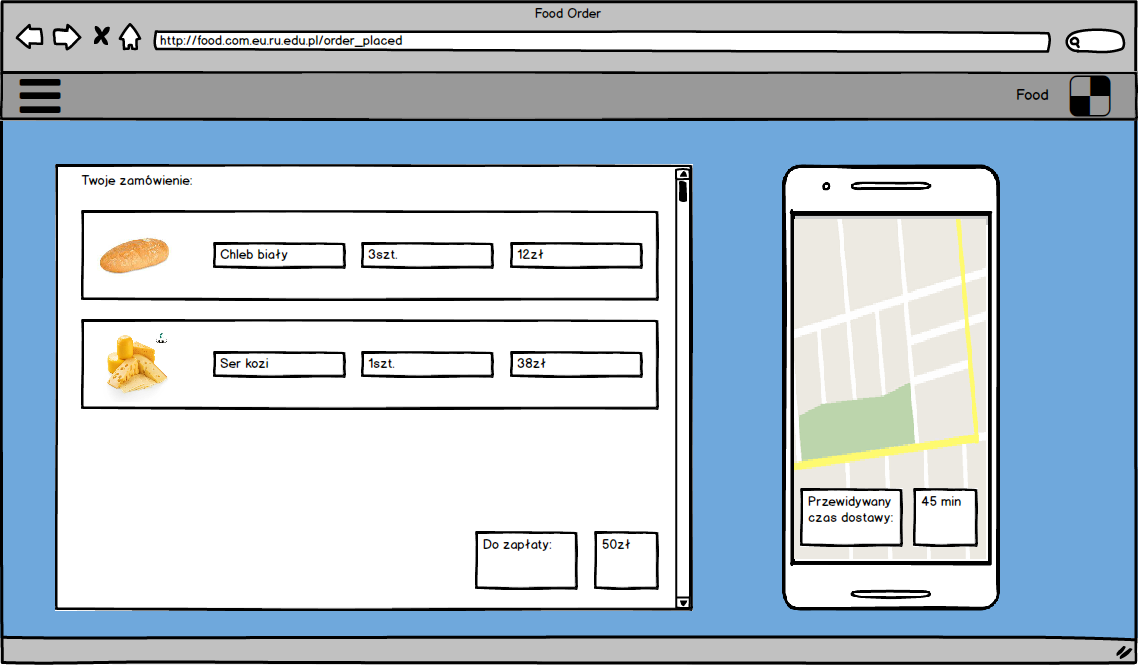
\includegraphics[width=15cm]{pictures/Zamowienie_zlozone_v3.png}
\caption{Ekran złożonego zamówienia.}
\end{figure}

\subsection{Uwagi zamawiającego}
Zamawiający prosił jeszcze o zmianę obrazu telefonu na ekranie logowania na bardziej współczesny, identyczny do tego, który widnieje na ekranie złożonego zamówienia oraz o przedstawienie ekranu śledzenia przesyłek.
